\chapter{Práctica 4: Caracterización de Circuitos con Diodos}

\section{Objetivos}
En esta práctica, vamos a obtener la relación entre la caída de tensión y la corriente en un diodo. Esto lo haremos estudiando el comportamiento de un diodo en un circuito sencillo.

\section{Fundamento Teórico}
La relación entre la caída de tensión y la corriente en un diodo viene dada por la siguiente expresión:
\begin{equation}\label{Ec:Rel_I-V}
    I = I_s \left( e^\frac{qV_d}{nkT} - 1\right)
\end{equation}
siendo:
\begin{itemize}
    \item $I$: La intensidad de la corriente que atraviesa el diodo.
    \item $V_d$: La diferencia de tensión entre los extremos del diodo.
    \item $I_s$: La corriente de saturación inversa, característica de cada diodo.
    \item $q$: La carga del electrón ($q = 1.6\cdot10^{-19}\;C$).
    \item $T$: La temperatura de la unión, característica de cada diodo. [$K$].
    \item $k$: La constante de Boltzmann ($k = 1.38 \cdot 10^-23\;J/K$).
    \item $n$: El índice de idealidad, que suele adoptar valores entre 1 (para el germanio) y del orden de 2 (para el silicio).
\end{itemize}

Debido a la complejidad de esa expresión, donde con frecuencia aparecerían ecuaciones trascendentales, se hace uso de dos métodos.

El primer método, reflejado en la figura \ref{fig:Met1}, indica que el diodo conduce o no en función de una tensión umbral, $V_\gamma$. Si conduce, este se sustituye por una fuente de tensión en serie con una resistencia; y en caso contrario se sustituye por un circuito abierto.

\begin{figure}
    \centering
    \[
        \begin{circuitikz}
            \draw (0,0) to [ empty diode] (1, 0);
        \end{circuitikz}
        = \left\{
            \begin{array}{lcc}
                \begin{circuitikz}
                    \draw (0,0)
                    to [short, -*] (0.4, 0)
                    to [open]  (1.6,0)
                    to [short, *-]  (2,0);
                \end{circuitikz}
                &   si  &   V_i < V_\gamma \\
                
                \begin{circuitikz}
                    \draw (0,0)
                    to [battery1, l=$V_\gamma$] (0.5, 0)
                    to [american resistor, l=$r_d$]  (2,0);
                \end{circuitikz}   &   si  &   V_i \geq V_\gamma
            \end{array}    
        \right.
    \]
        
    \[
        I_d= \left\{
        \begin{array}{lcc}
            0 &   si  &   V_i < V_\gamma \\
            \frac{V_d}{r_d}   &   si  &   V_i \geq V_\gamma
        \end{array}    
        \right.
    \]

    \[
        V_d= \left\{
        \begin{array}{lcc}
            V_i &   si  &   V_i < V_\gamma \\
            \frac{r_d}{r_d+R}\;V_i + \frac{R\;V_\gamma}{r_d+R}  &   si  &   V_i \geq V_\gamma
        \end{array}    
        \right.
    \]
    
    \caption{Método 1 de simplificación}
    \label{fig:Met1}
\end{figure}

El segundo método, aun más sencillo y reflejado en la figura \ref{fig:Met2}, indica igualmente que el diodo conduce o no en función de una tensión umbral, $V_\gamma$. Este método indica que, si el diodo conduce, este se sustituye por una fuente de tensión; y en caso contrario se sustituye por un circuito abierto.

\begin{figure}
    \centering
    \[
        \begin{circuitikz}
            \draw (0,0) to [ empty diode] (1, 0);
        \end{circuitikz}
        = \left\{
            \begin{array}{lcc}
                \begin{circuitikz}
                    \draw (0,0)
                    to [short, -*] (0.2, 0)
                    to [open]  (0.8,0)
                    to [short, *-]  (1,0);
                \end{circuitikz}
                &   si  &   V_i < V_\gamma \\
                
                \begin{circuitikz}
                    \draw (0,0)
                    to [battery1, l=$V_\gamma$] (1, 0);
                \end{circuitikz}   &   si  &   V_i \geq V_\gamma
            \end{array}    
        \right.
    \]
        
    \[
        I_d= \left\{
        \begin{array}{lcc}
            0 &   si  &   V_i < V_\gamma \\
            V_d   &   si  &   V_i \geq V_\gamma
        \end{array}    
        \right.
    \]

    \[
        V_d= \left\{
        \begin{array}{lcc}
            V_i &   si  &   V_i < V_\gamma \\
            V_\gamma  &   si  &   V_i \geq V_\gamma
        \end{array}    
        \right.
    \]
    
    \caption{Método 2 de simplificación}
    \label{fig:Met2}
\end{figure}

Para estudiar el comportamiento del diodo, vamos a montar el circuito de la figura \ref{fig:Circuito} y representaremos la característica de transferencia tomando como entrada $V_i$ y como salida $V_0(=V_d)$.

\begin{figure}
    \centering
    \begin{circuitikz}
        \draw (0, 0) to [battery1, a=$V_i$] (0,-2)
        (0,0) to [american resistor, l=$R$] (2.5, 0)
        to [short] (2.8,0)
        (2.5, 0) to [empty led, l=D]  (2.5,-2)
        to [short]  (0, -2);

        \draw (2.8,0) node [right] {$V_0$}
        (2.5, -2) node [ground] {};
    \end{circuitikz}
    \caption{Montaje Experimental}
    \label{fig:Circuito}
\end{figure}


\section{Material}
\begin{itemize}
    \item \underline{Fuente de alimentación:} fuente de tensión de corriente continua empleada para proporcionarle tensión al circuito. El modelo empleado es FAC-363B.
    \item \underline{Polímetro digital:} dispositivo empleado para realizar diversas medidas en el circuito. Es usado principalmente en corriente continua para medir la resistencia, diferencia de potencial o capacidad de un condensador, por ejemplo.
    \item \underline{Resistencia}
    \item \underline{Diodo LED} diodo que se ilumina cuando conduce. En la figura \ref{fig:LED} se aprecia que la patilla larga es la parte P.
    \begin{figure}[H]
        \centering
        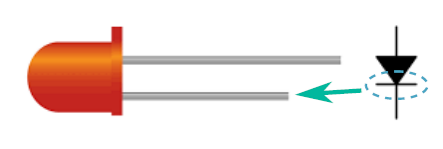
\includegraphics[height=1.5 cm]{Imágenes 04/LED.png}
        \caption{Diodo Led}
        \label{fig:LED}
    \end{figure}
    \item \underline{Protoboard}
\end{itemize}


\section{Desarrollo y resultados}
El valor de la resistencia empleada en el circuito es:
\begin{itemize}
    \item $R = 992\;\Omega$
\end{itemize}
Una vez medidos estos, se han medido diversas magnitudes conforme se variaba el valor de $V_i$, el potencial de entrada. Los datos obtenidos se muestran en la figura \ref{fig:Datos}, donde cada columna representa:
\begin{description}
    \item [Columna 1:] Potencial de entrada teórico ($V_i^{teo}$) [$V$]. Dado por la fuente de alimentación.
    \item [Columna 2:] Potencial de entrada real ($V_i^{exp}$) [$V$]. Medido con el polímetro.
    \item [Columna 3:] Caída de potencial en el diodo [$V$]. Medido con el polímetro.
    \item [Columna 4:] Caída de potencial en la resistencia [$V$]. Medido con el polímetro.
    \item [Columna 5:] Intensidad que circula por la malla [$A$]. Calculada como $I = \frac{V_r}{R}$
\end{description}
\newpage

\begin{figure}
    \centering
    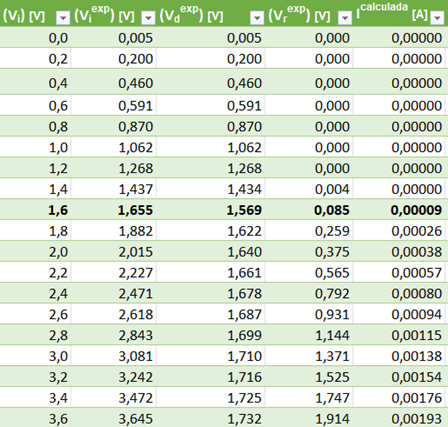
\includegraphics[width=10cm]{Imágenes 04/Tabla_Datos_Exp.png}
    \caption{Datos obtenidos en el circuito de la figura \ref{fig:Circuito}.}
    \label{fig:Datos}
\end{figure}

En la figura \ref{fig:Rel_I-V} se observa cómo varía la intensidad de un circuito en función de $V_d$. Solo se representan los valores para los que el diodo conduce.

\begin{figure}
    \centering
    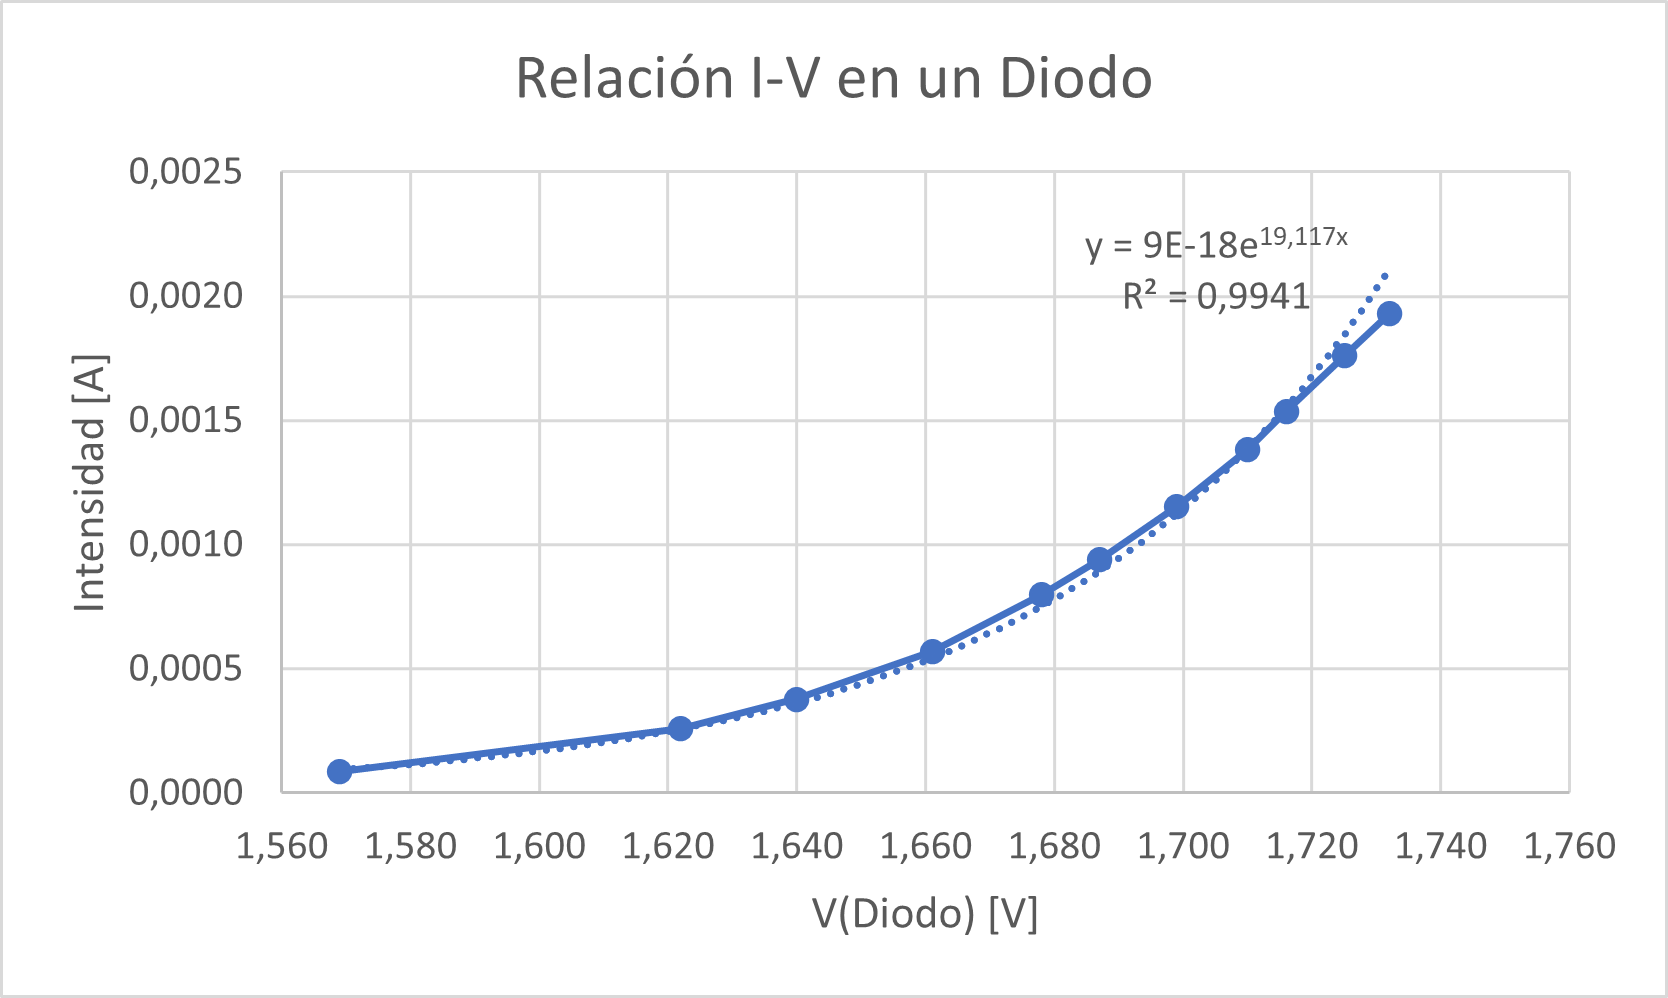
\includegraphics[width=13cm]{Imágenes 04/Rel_I-V.png}
    \caption{Relación I-V en un diodo.}
    \label{fig:Rel_I-V}
\end{figure}

En la figura \ref{fig:Car_Trans} se muestra la característica de de transferencia del circuito tomando como entrada el potencial suministrado por la fuente de tensión y como salida la caída de voltaje en el diodo.

\begin{figure}
    \centering
    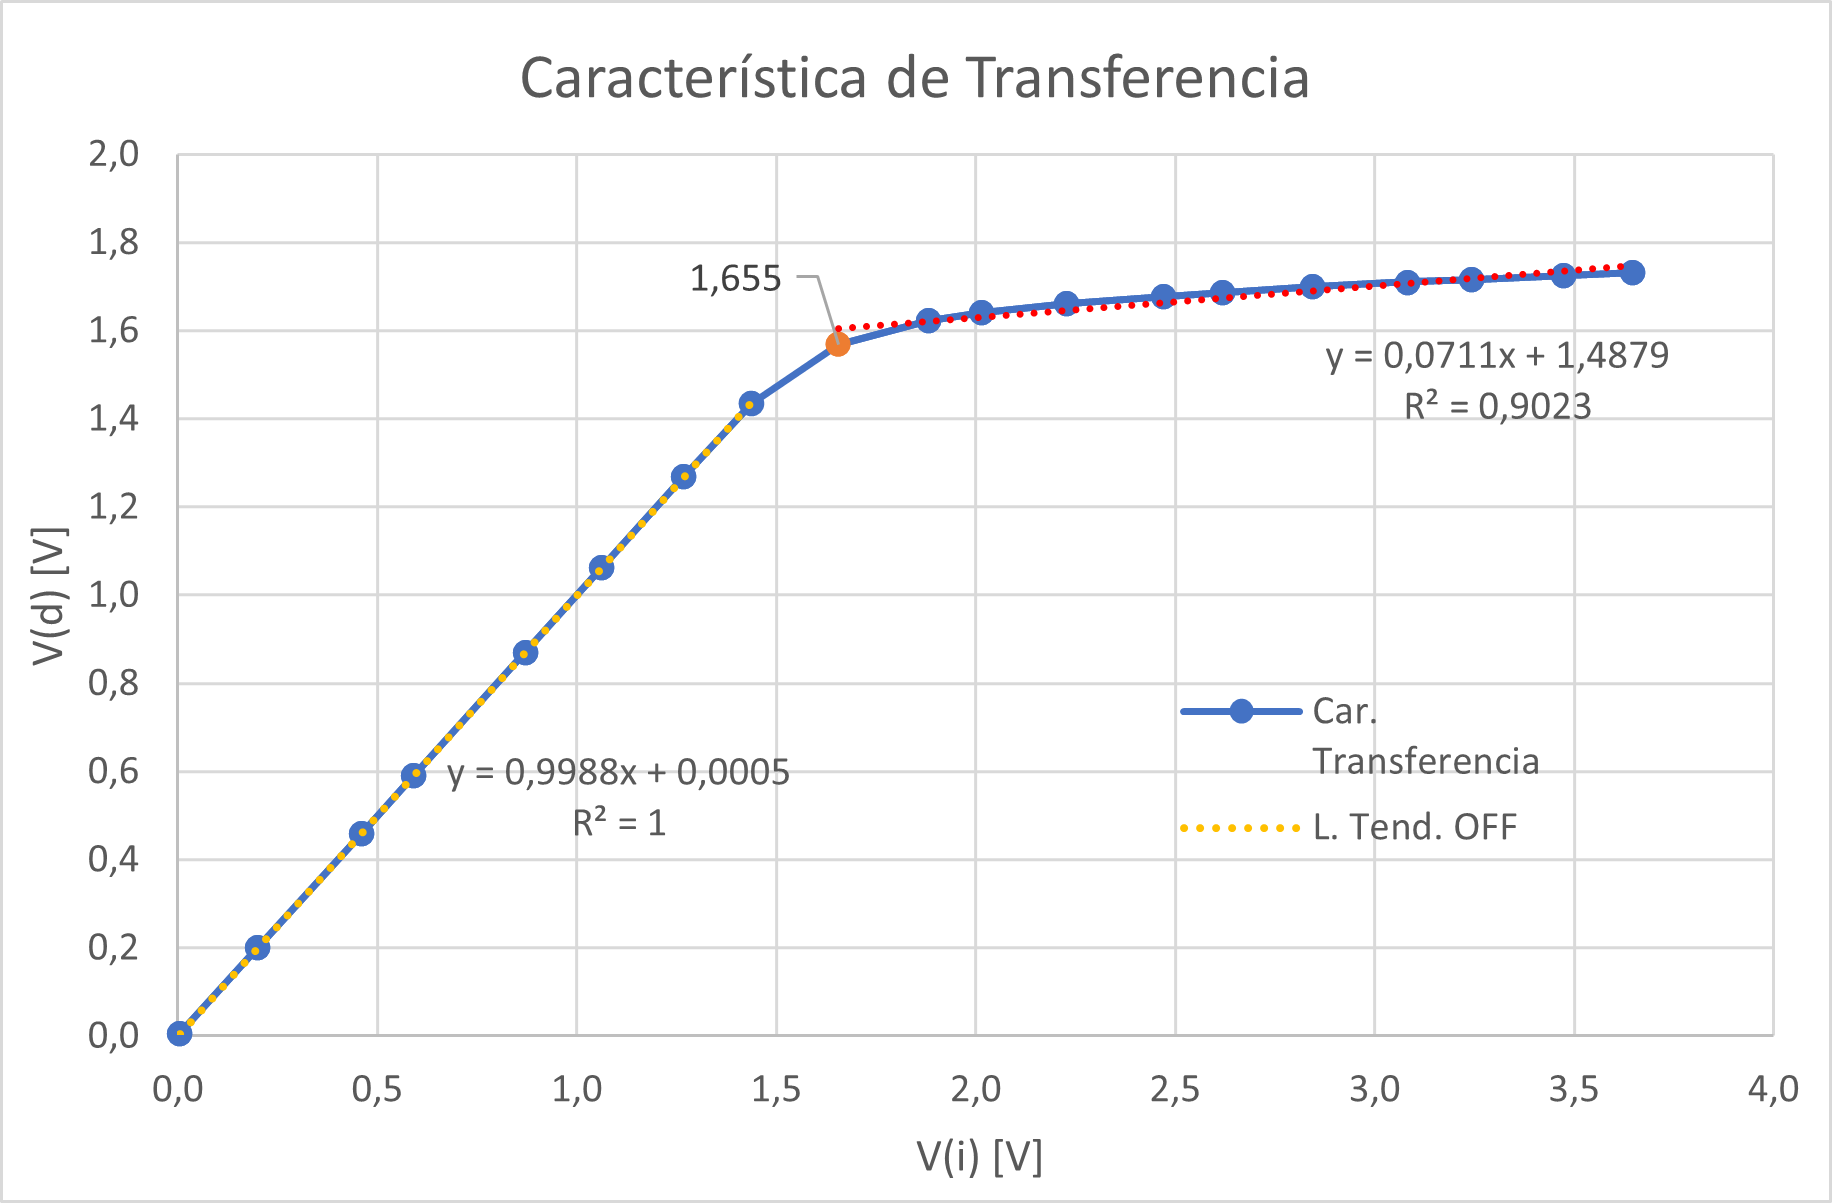
\includegraphics[width=13cm]{Imágenes 04/Car_Trans.png}
    \caption{Característica de transferencia del circuito tomando como salida $V_d$.}
    \label{fig:Car_Trans}
\end{figure}




\section{Discusión}

\subsection{Curva I-V en un diodo}

En primer lugar, se ha representado la intensidad que circula por un diodo frente a la caída de potencial en este (figura \ref{fig:Rel_I-V}). Solo se han representado los valores para los que circula corriente, ya que para evitar resolver ecuaciones trascendentales vamos a aproximar la expresión teórica:
\begin{equation}
    I_d \approx I_s\;e^\frac{qV_d}{nkT}
\end{equation}

Tras obtener la linea de tendencia exponencial\footnote{Coef. de correlación $R^2 = 0.9941$ cercano a 1, luego el ajuste es suficientemente preciso.}, vemos que:
\begin{equation}
    I_d \approx I_s\;e^\frac{qV_d}{nkT} \approx 9\cdot 10^{-18} e^{19.117V_d}
\end{equation}

Por tanto,
\begin{itemize}
    \item $I_s = 9\cdot 10^{-18} \; A$
    \item $\frac{q}{nkT} = 19.117$. Como $T=19^\circ C = 292.15\;K$,
        $$
            n = \frac{q}{kT\cdot 19.117} = 2.07
        $$
\end{itemize}

Como vemos, $n\approx 2$, lo que nos indica que el diodo LED posiblemente sea de silicio. Los resultados obtenidos concuerdan con la teoría ya que la relación se ajusta de manera correcta ($R^2\approx 1$) a la relación I-V definida en la Ec. \ref{Ec:Rel_I-V}.

\subsection{Estudio de la bondad de los modelos de aproximación}
A partir de la figura \ref{fig:Datos}, vemos que, para este diodo, $V_\gamma \approx 1.6\;V$. Por tanto, se representa la característica de transferencia tomando como salida $V_d$ y se obtienen las tendencias lineales de ambos tramos, cuando el diodo está encendido y cuando está apagado. Estos resultados se encuentran en la figura \ref{fig:Car_Trans}.

\begin{description}
    \item[Si $\mathbf{V_i < V_\gamma}$] En este caso $I=0 A$, luego el diodo está apagado. Diodo OFF.\\
    \begin{equation}
        V_d = 0.9988 \;V_i + 0.0005
    \end{equation}
    Como $R^2=1$, el ajuste es prácticamente perfecto.
    \begin{enumerate}
        \item \textbf{Modelo 1} (Figura \ref{fig:Met1}).\\
        Este modelo afirma que, en este caso, $V_d = V_i$, ya que el diodo se sustituye por un circuito abierto por lo que no circula corriente. Como $m=0.9988\approx1$ y $n=0.0005\approx0$, este modelo es válido en este tramo, ya que los resultados que predice teóricamente se ajustan muy fiablemente a lo que ocurre en la realidad.
        \item \textbf{Modelo 2} (Figura \ref{fig:Met2}).\\
        Como en este caso afirma lo mismo que en el primer modelo, este es igualmente válido.
    \end{enumerate}

    \item[Si $\mathbf{V_i \geq V_\gamma}$] En este caso $I\neq0 A$, luego el diodo está encendido. Diodo ON.\\
    \begin{equation}
        V_d = 0.0711\;V_i + 1.4879
    \end{equation}
    Como $R^2 = 0.9023$, el ajuste no es ideal pero los resultados serán coherentes.
    \begin{enumerate}
        \item \textbf{Modelo 1} (Figura \ref{fig:Met1}).\\
        Este modelo afirma que, en este caso, $V_d = \frac{r_d}{r_d+R}\;V_i + \frac{R\;V_\gamma}{r_d+R}$.
        Por tanto,
        $$
            \frac{V_\gamma \; R}{r_d + R} = 1.4879 \Longrightarrow r_d = 1.4879\;\frac{R+r_d}{R} = 75.92\;\Omega
        $$
        $$
            \frac{r_d}{r_d + R} = 0.0711 \Longrightarrow V_\gamma = 0.0711\;\frac{R}{1-0.0711} = 1.601\; V
        $$
        
        Por tanto, con $r_d = 75.92\;\Omega$ y $V_\gamma = 1.601\;V$ este modelo se ajusta a lo que ocurre en la realidad, ya que coincide con la linea de tendencia. Además, Se cumple que $V_\gamma \approx 1.6\;V$, como habíamos predicho.
        
        \item \textbf{Modelo 2} (Figura \ref{fig:Met2}).\\
        Este modelo afirma que, en este caso, $V_d = V_\gamma$.
        Por tanto, este modelo es válido solo si $0.0711\approx 0$ y $1.4879 \approx V_\gamma$. Como vemos, este modelo se ajusta peor a la realidad, ya que no es una recta totalmente horizontal (como predice esta simplificación) sino que tiene cierta pendiente. Esto provoca también que $V_\gamma$ sea mayor que la que este modelo predice.
    \end{enumerate}
    
\end{description}


\section{Conclusiones}
Las conclusiones extraídas de esta práctica de laboratorio son:
\begin{itemize}
    \item En primer lugar, podemos ver que gracias a la investigación se tienen modelos de simplificación que, aunque no representan perfectamente lo que ocurre en realidad, nos aportan resultados coherentes, fiables y similares a los reales facilitándonos en gran medida los cálculos, por lo que son muy útiles.
    
    \item En base a los resultados obtenidos, también se puede deducir que, existe un valor umbral, $V_\gamma$, a partir del cual el diodo pasa a conducir una corriente insignificante a conducir de manera proporcional a la diferencia de potencial. Además, en la característica de transferencia también se aprecia a la perfección que, una vez el diodo conduce, la caída de potencial en sus extremos se estabiliza en cierta medida en ese valor umbral.

    \item Por último, se ha podido comprobar la característica del diodo como \emph{semiconductor}, ya que en función del potencial de entrada se ha podido observar que conduce o no.
\end{itemize}